\documentclass[11pt]{article}

\usepackage[margin=1in]{geometry}
\usepackage{graphicx}
\usepackage{amsmath,amssymb}
\usepackage{booktabs}
\usepackage{hyperref}
\usepackage{caption}
\usepackage{float}
\usepackage{siunitx}
\usepackage{enumitem}

\hypersetup{
  colorlinks=true,
  linkcolor=blue,
  citecolor=blue,
  urlcolor=blue
}

\title{\textbf{Multimodal Mersivity (Milestones 1 \& 2)}\\
\large Sonification and Time--Frequency Visualization of Cognitive States from EEG}
\author{Harsanjam Saini}
\date{\today}

\begin{document}
\maketitle

\begin{abstract}
This report documents Milestones 1 and 2 of the \emph{Multimodal Mersivity} project: a reproducible EEG processing workflow that converts pre-recorded EEG into (i) cleaned band-limited features for cognitive-state modeling and (ii) low-latency auditory feedback via sonification. Milestone 1 covers literature on auditory display/sonification, EEG preprocessing and feature extraction for alpha, beta, and theta activity, and time--frequency analysis methods (Fourier/STFT and wavelets), with optional background on chirplet-based methods. Milestone 2 presents an end-to-end parameter-mapping sonification framework and benchmarks responsiveness on streaming-style sliding windows. The pipeline produces diagnostic PSD plots, time--frequency visualizations (STFT spectrogram and Morlet wavelet scalogram), time-resolved bandpower trajectories, optional calm vs.\ stress classification baselines, and an exported WAV sonification.
\end{abstract}

\section{Project background and objective}
Conventional EEG displays (raw traces, numeric summaries, spectra) can be effective for expert analysis but are less accessible to non-specialists. Auditory display and sonification provide an alternative perceptual channel for monitoring temporal dynamics, potentially reducing reliance on visual attention while supporting an immersive ``Mersivity'' experience \cite{hermann2011}. The objective of Milestones 1 and 2 is to establish a robust signal processing and sonification backbone: acquire (or support acquisition of) an EEG dataset, implement reproducible preprocessing and feature extraction, compare Fourier/STFT with wavelet time--frequency analyses, and build a responsive sonification pipeline where EEG features drive pitch, loudness, and modulation.

\section{Milestone 1: Literature review (focused)}
\subsection{EEG sonification and auditory displays}
The Sonification Handbook provides a comprehensive treatment of auditory display principles and practical designs, including \emph{parameter mapping sonification}, in which data variables are mapped to auditory parameters such as pitch, loudness, timbre, and spatialization \cite{hermann2011}. For EEG, parameter mapping is often preferred for interpretability: changes in bandpower or ratios can be linked to audible shifts in pitch or brightness, enabling intuitive, real-time tracking of cognitive-state proxies.

\subsection{EEG preprocessing and band-limited features}
EEG recordings are affected by slow drift, high-frequency noise, and powerline interference; preprocessing therefore typically includes band-pass filtering and notch filtering, alongside referencing strategies and artifact handling (e.g., robust clipping, rejection, or ICA depending on constraints) \cite{cohen2014}. Canonical band activity---especially theta (\SIrange{4}{8}{Hz}), alpha (\SIrange{8}{13}{Hz}), and beta (\SIrange{13}{30}{Hz})---is frequently summarized via bandpower features for downstream modeling and visualization \cite{cohen2014}.

\subsection{Time--frequency analysis: STFT vs.\ wavelets}
Time--frequency methods characterize how spectral content evolves over time. The short-time Fourier transform (STFT) computes spectra on sliding windows, providing straightforward interpretation and efficient computation, but it exhibits a fixed time--frequency resolution determined by the window length. Wavelet methods (e.g., Morlet CWT) provide multi-resolution analysis: higher temporal resolution at higher frequencies and higher spectral resolution at lower frequencies, often improving interpretability for transient oscillatory events \cite{cohen2014}. This milestone includes a direct empirical comparison on representative EEG segments.

\subsection{Optional background: chirplet-based methods}
Chirplet transforms generalize time--frequency atoms to include chirp rate (time-varying instantaneous frequency), allowing improved representation of nonstationary, chirping components \cite{mann1995}. While not implemented here (optional per milestone specification), chirplets provide a useful conceptual extension when EEG rhythms display systematic frequency sweeps or nonstationary structure.

\section{Milestone 1: Data acquisition and preprocessing}
\subsection{Dataset acquisition}
For milestone compliance, the pipeline supports public EEG datasets such as DEAP, a multimodal dataset with EEG recordings and per-trial affect ratings (including arousal), enabling a reasonable proxy labeling strategy for calm vs.\ stress via low vs.\ high arousal thresholds \cite{koelstra2012}. Due to distribution constraints, the repository includes a converter (\texttt{scripts/deap\_to\_csv.py}) to transform downloaded DEAP subject files into the project CSV format.

For immediate end-to-end validation, we also include a synthetic labeled EEG session that emulates calm vs.\ stress by modulating alpha and beta amplitudes. This enables deterministic reproduction of the pipeline and its figures.

\subsection{Reproducible preprocessing pipeline}
Given an input CSV recording, the preprocessing stage applies:
\begin{itemize}[leftmargin=2em]
  \item \textbf{Detrending} to reduce slow baseline drift.
  \item \textbf{Robust clipping} (MAD-based winsorization) as basic artifact handling.
  \item \textbf{Band-pass filtering} (\SIrange{1}{45}{Hz}) to isolate canonical EEG rhythms.
  \item \textbf{Notch filtering} at mains frequency (\SI{50}{Hz} or \SI{60}{Hz}) (and harmonic if in-band).
  \item \textbf{Average re-referencing} (optional) to reduce common-mode activity.
\end{itemize}

A PSD sanity check before vs.\ after preprocessing is shown in Figure~\ref{fig:psd}.

\begin{figure}[H]
  \centering
  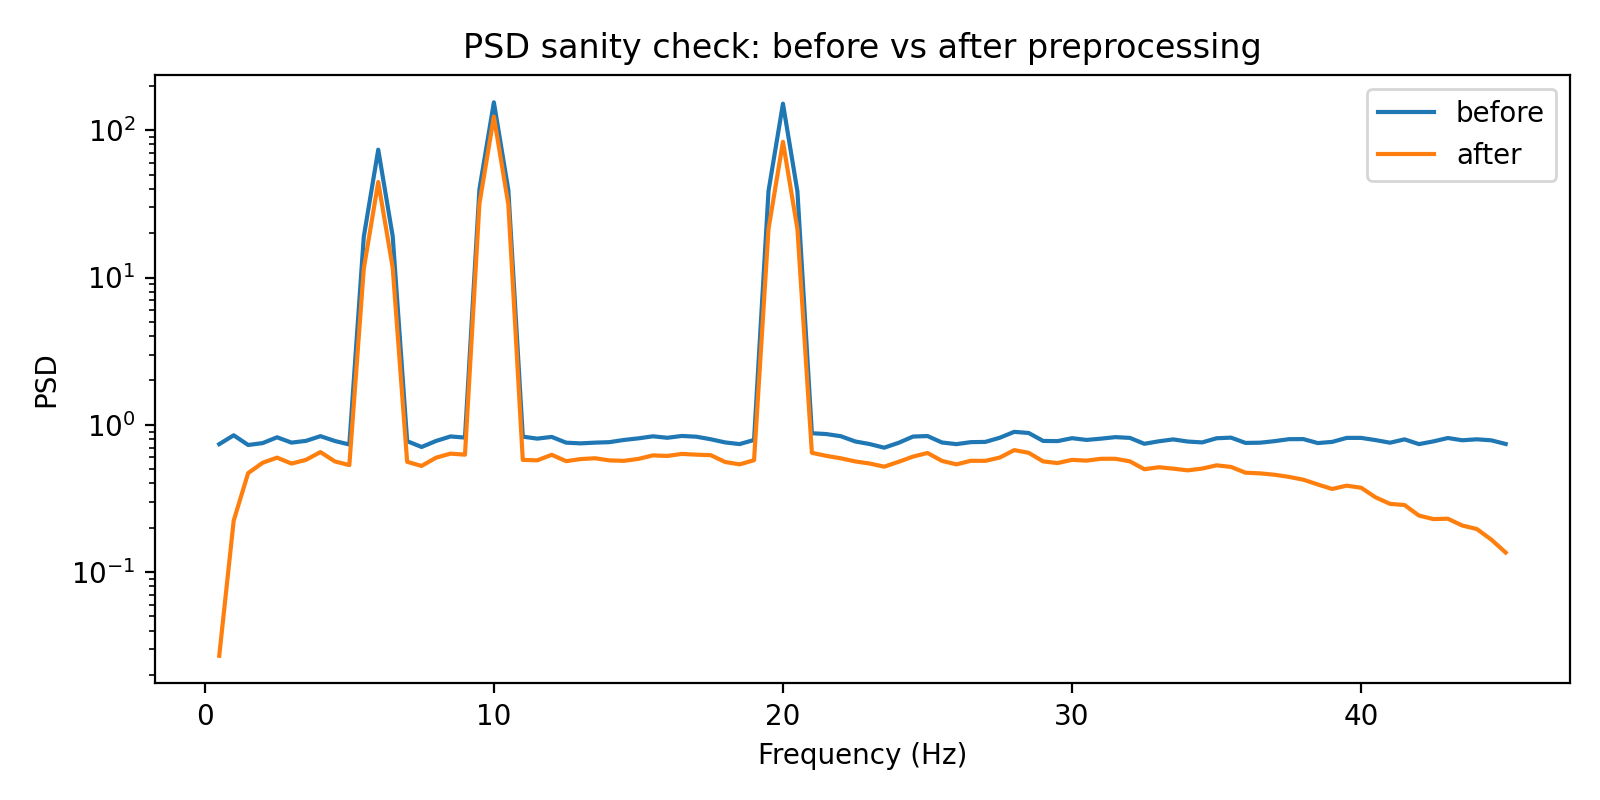
\includegraphics[width=0.95\linewidth]{figures/psd_before_after.png}
  \caption{PSD sanity check: mean PSD before vs.\ after preprocessing.}
  \label{fig:psd}
\end{figure}

\subsection{Feature extraction (alpha/beta/theta bandpower)}
Features are computed on sliding windows of length $W$ with hop size $H$. For each window, we estimate power spectral density using Welch-style averaging and integrate power within standard bands (delta/theta/alpha/beta/gamma). In addition to absolute bandpower, ratio features such as $\mathrm{beta}/\mathrm{alpha}$ are included for compact arousal proxies.

Time-resolved bandpower trajectories are shown in Figure~\ref{fig:band}.

\begin{figure}[H]
  \centering
  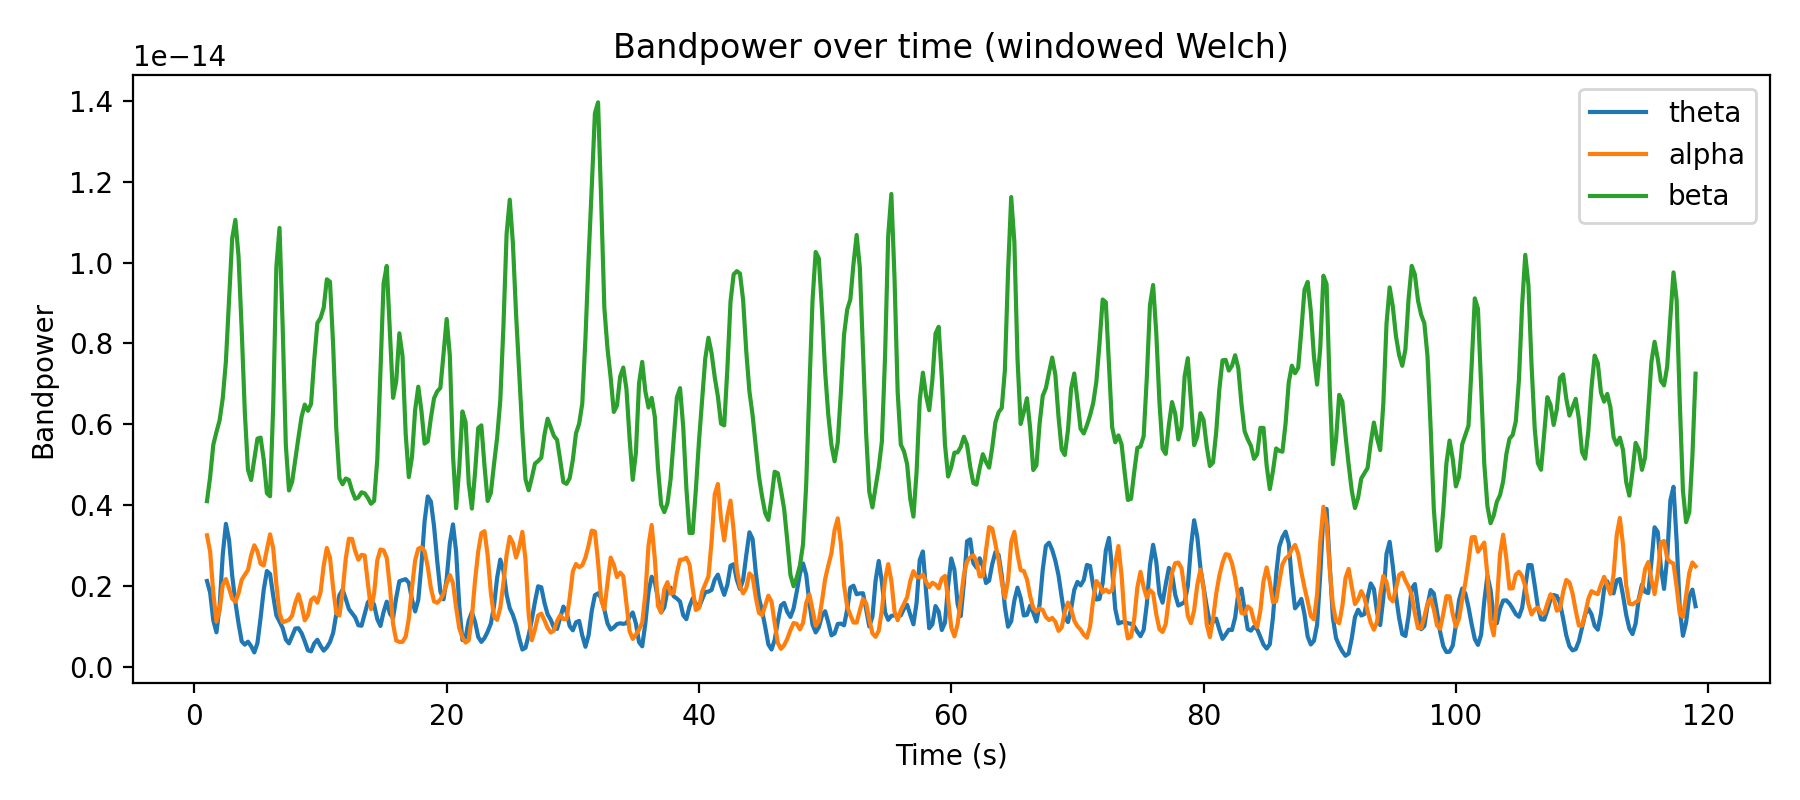
\includegraphics[width=0.95\linewidth]{figures/bandpowers.png}
  \caption{Windowed bandpower over time (theta/alpha/beta).}
  \label{fig:band}
\end{figure}

\subsection{Fourier/STFT vs.\ wavelet comparison}
Figures~\ref{fig:stft} and \ref{fig:wavelet} compare STFT and Morlet wavelet scalograms on the same representative EEG segment. Both reveal the dominant rhythmic components, while wavelets offer multi-resolution behavior (finer temporal structure at higher frequencies). Computational timing on the same segment is summarized in Table~\ref{tab:tf}.

\begin{figure}[H]
  \centering
  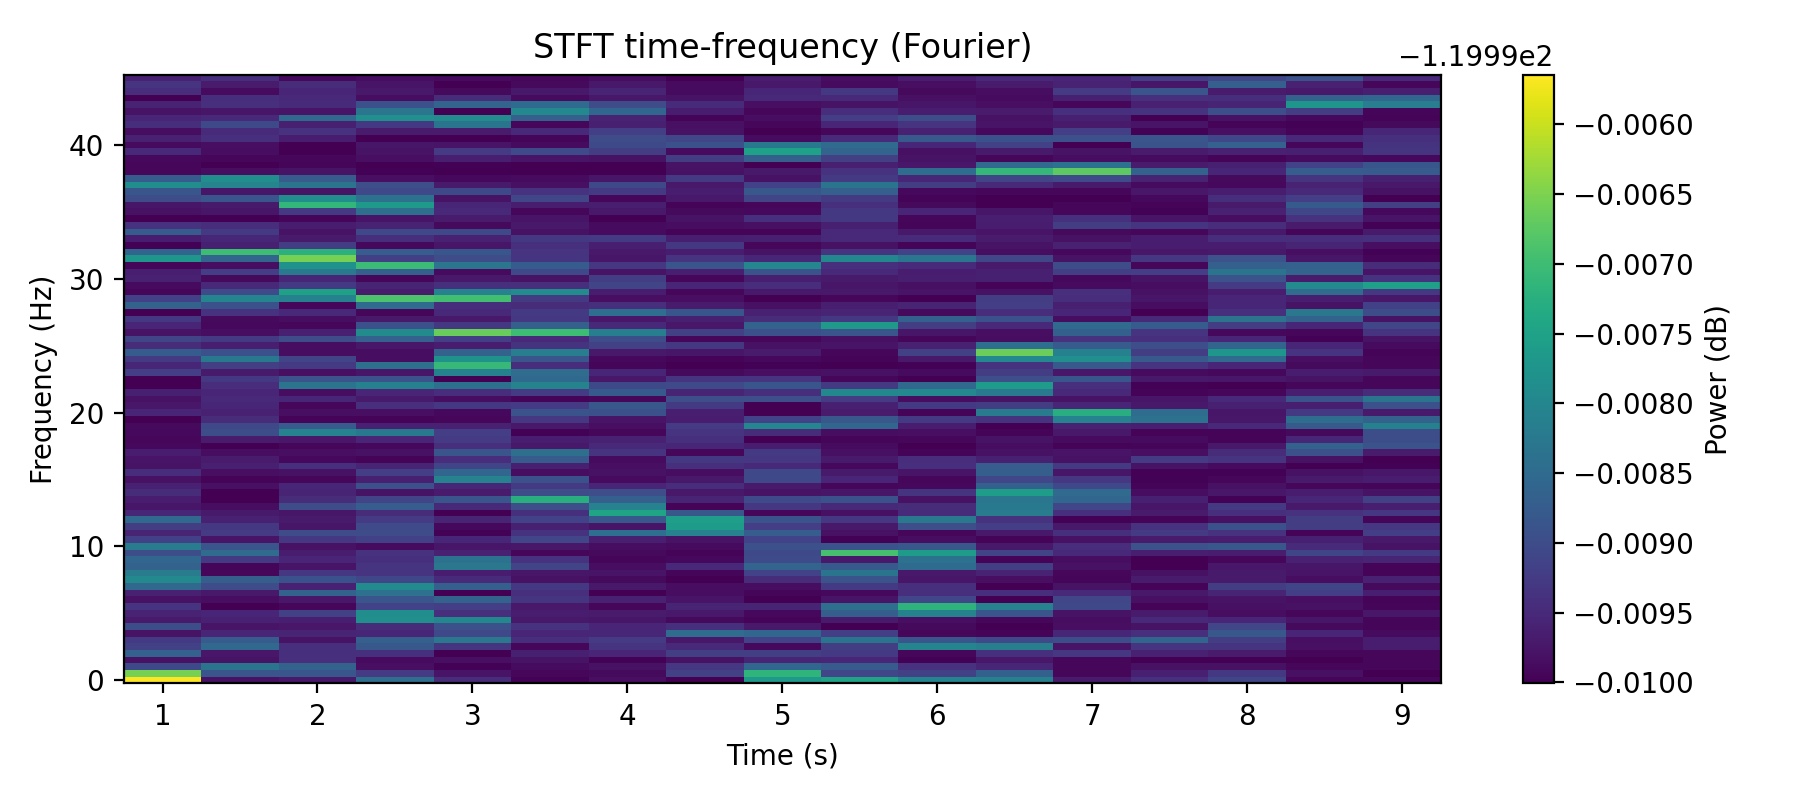
\includegraphics[width=0.95\linewidth]{figures/tf_stft.png}
  \caption{STFT time--frequency representation (Fourier-based).}
  \label{fig:stft}
\end{figure}

\begin{figure}[H]
  \centering
  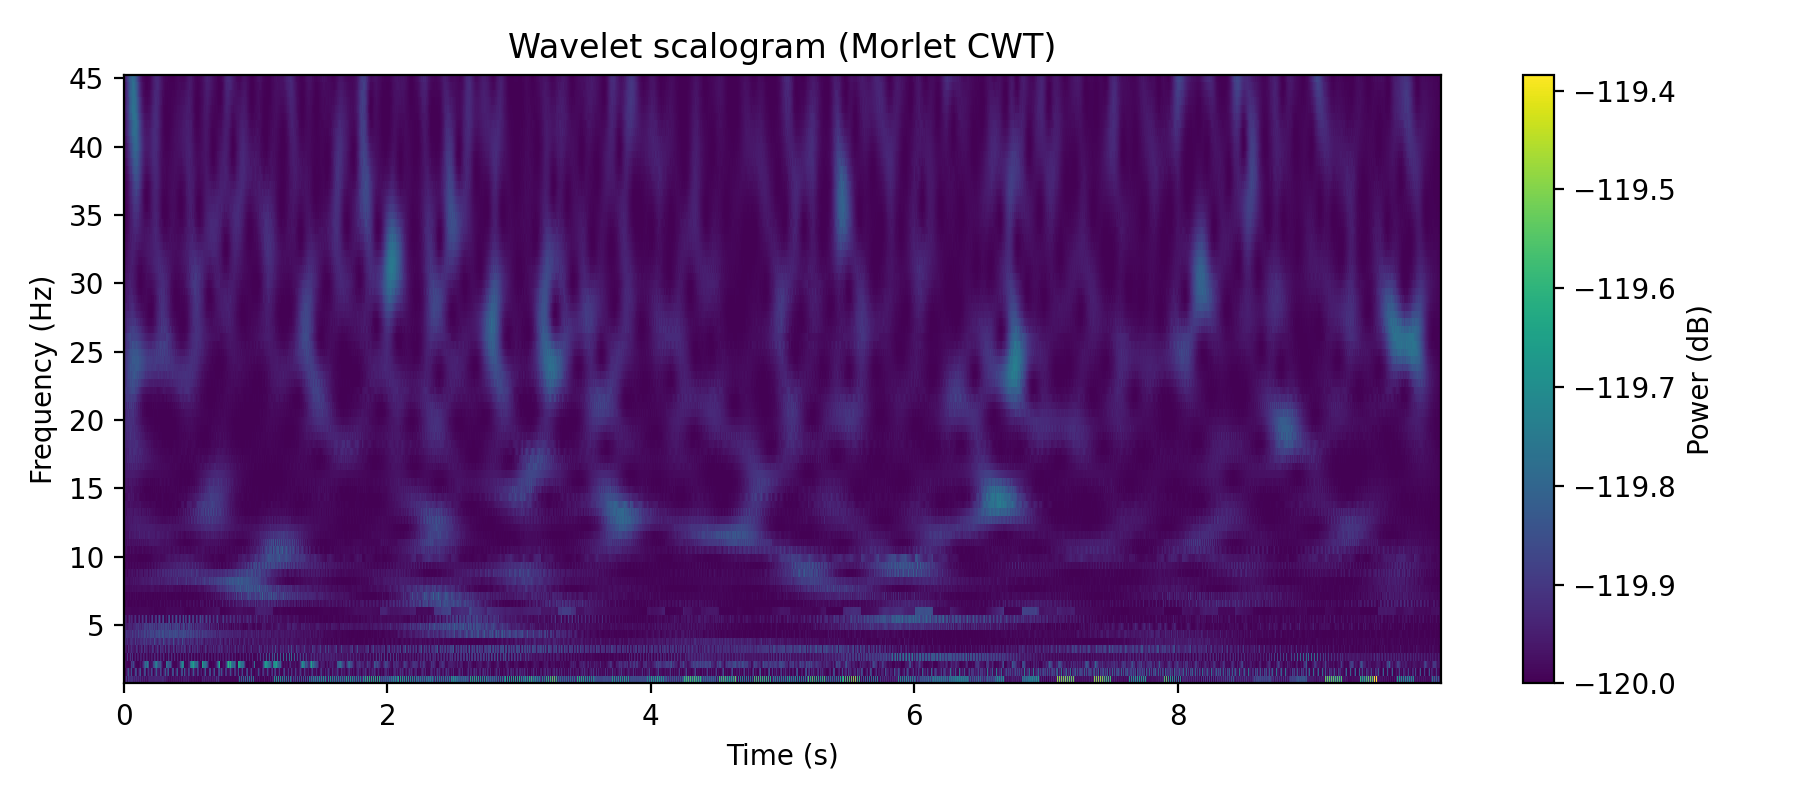
\includegraphics[width=0.95\linewidth]{figures/tf_wavelet.png}
  \caption{Morlet wavelet scalogram (CWT).}
  \label{fig:wavelet}
\end{figure}

\begin{table}[H]
\centering
\caption{Time--frequency computation time on a representative segment.}
\label{tab:tf}
\begin{tabular}{lrr}
\toprule
Method & Time (ms) & Notes \\
\midrule
STFT (windowed FFT) & 0.81 & Fixed resolution (window-controlled) \\
Morlet CWT (wavelet) & 29.09 & Multi-resolution; higher compute cost \\
\bottomrule
\end{tabular}
\end{table}

\section{Milestone 2: Sonification pipeline and responsiveness}
\subsection{Parameter mapping design}
Following parameter mapping principles \cite{hermann2011}, we map normalized EEG features to auditory controls:
\begin{itemize}[leftmargin=2em]
  \item \textbf{Pitch} $\leftarrow$ alpha power (higher alpha $\Rightarrow$ higher pitch).
  \item \textbf{Brightness/timbre} $\leftarrow$ beta/alpha ratio (higher ratio $\Rightarrow$ stronger saturation/noise).
  \item \textbf{Vibrato depth} $\leftarrow$ theta power.
  \item \textbf{Amplitude} $\leftarrow$ total normalized power.
\end{itemize}
Pitch is quantized to a scale to stabilize perception; calm windows use a major scale and stress windows use a minor scale in the baseline implementation. The audio stream is rendered offline as a WAV file (\texttt{sonification.wav}), one audio segment per hop.

\subsection{Responsiveness benchmarking}
To evaluate responsiveness, we measure per-hop compute time for key feature calculations in a streaming-style loop. For hop size $H = 0.25$~s, the measured mean compute time is 0.96~ms and the 95th percentile is 1.09~ms, corresponding to a real-time factor of approximately 261.4$\\times$ (values $>1$ indicate the pipeline is faster than real time at the chosen hop).

\begin{figure}[H]
  \centering
  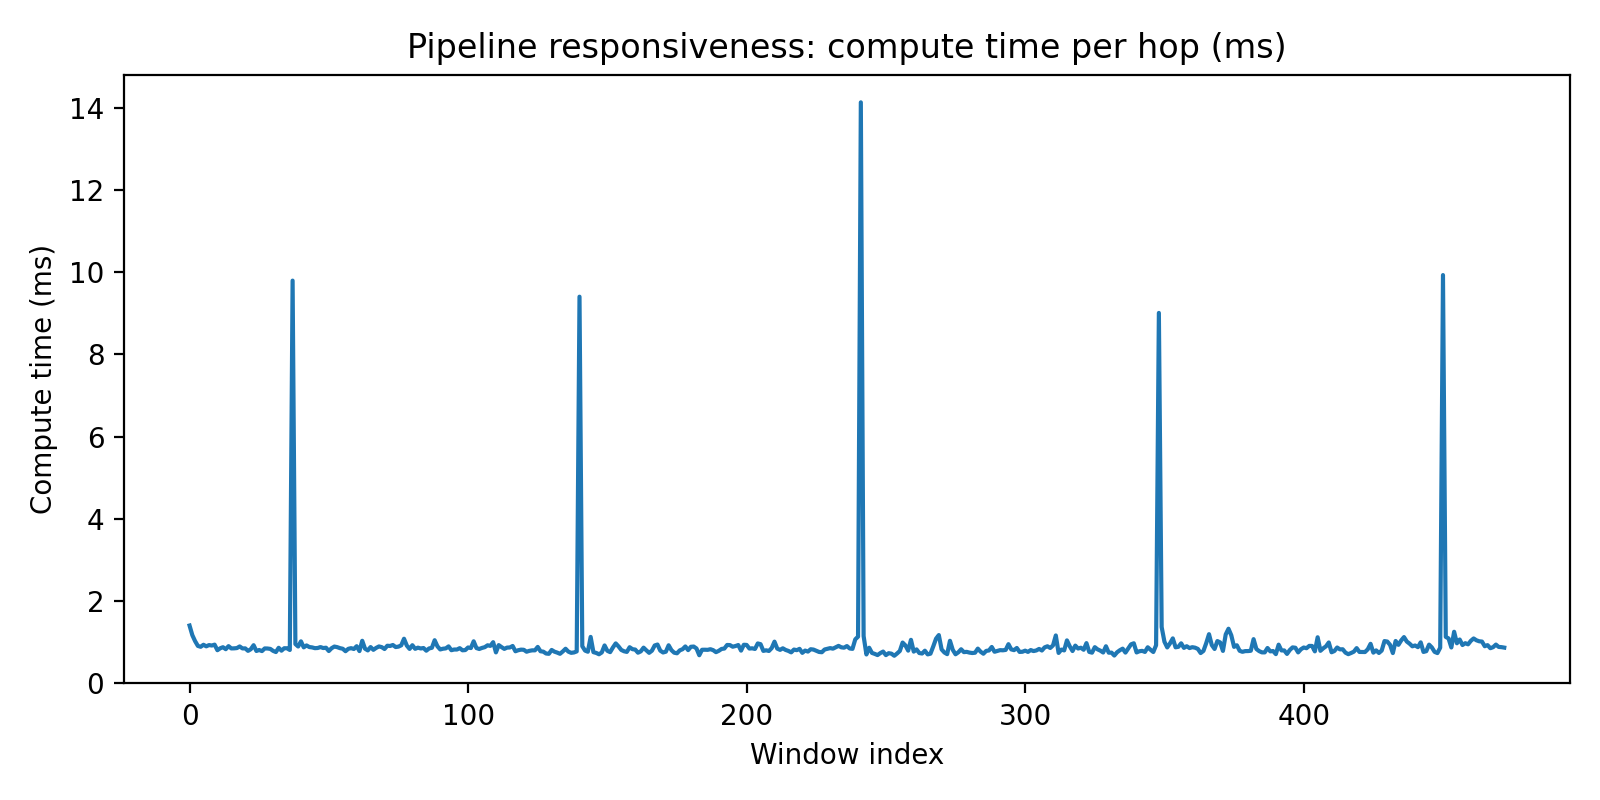
\includegraphics[width=0.95\linewidth]{figures/latency_ms.png}
  \caption{Per-hop compute time (ms) during streaming-style feature extraction (responsiveness).}
  \label{fig:lat}
\end{figure}

\subsection{Optional baseline: calm vs.\ stress classification}
When labels are present, a lightweight logistic regression classifier can be trained on bandpowers and ratios to provide a sanity-check baseline for calm vs.\ stress discrimination. The resulting confusion matrix is shown in Figure~\ref{fig:cm}. (This is a baseline for driving/being driven by audio modulation, not a clinical claim.)

\begin{figure}[H]
  \centering
  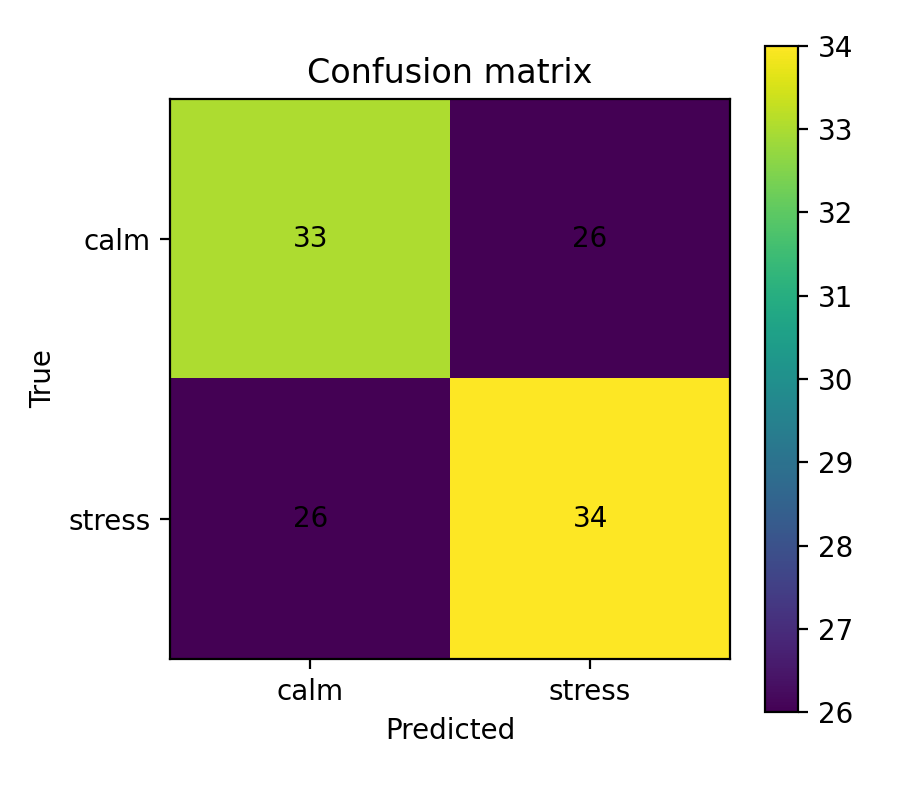
\includegraphics[width=0.70\linewidth]{figures/confusion_matrix.png}
  \caption{Example confusion matrix for calm vs.\ stress classification on windowed features.}
  \label{fig:cm}
\end{figure}

\section{Discussion and limitations}
Milestones 1 and 2 establish a reliable DSP and sonification backbone. The primary limitations are (i) simple artifact handling (robust clipping rather than ICA), (ii) potential label ambiguity and temporal misalignment in affective labeling, and (iii) evaluation concerns when splitting highly correlated adjacent windows. These issues will be addressed in later milestones via improved enhancement, more rigorous evaluation (session/subject splits), and multimodal visualization integration (SWIM-inspired geometric flow).

\section{Conclusion}
We delivered Milestone 1 and 2 requirements: a literature-informed EEG preprocessing and feature pipeline, explicit STFT vs.\ wavelet time--frequency comparison, and a responsive parameter-mapping sonification framework that exports a WAV representation of EEG-derived cognitive-state proxies. This provides the foundation for Milestone 3 (synchronized SWIM-style visualization + sonification) and Milestone 4 (signal enhancement and psychoacoustic refinement).

\begin{thebibliography}{9}

\bibitem{hermann2011}
T.~Hermann, A.~Hunt, and J.~G. Neuhoff (Eds.).
\newblock \emph{The Sonification Handbook}.
\newblock Logos Verlag Berlin, 2011. Available: sonification.de/handbook.

\bibitem{cohen2014}
M.~X. Cohen.
\newblock \emph{Analyzing Neural Time Series Data: Theory and Practice}.
\newblock MIT Press, 2014.

\bibitem{mann1995}
S.~Mann and S.~Haykin.
\newblock The chirplet transform: Physical considerations.
\newblock \emph{IEEE Transactions on Signal Processing}, 43(11):2745--2761, 1995.

\bibitem{koelstra2012}
S.~Koelstra et al.
\newblock DEAP: A Database for Emotion Analysis Using Physiological Signals.
\newblock \emph{IEEE Transactions on Affective Computing}, 3(1):18--31, 2012.

\end{thebibliography}

\end{document}
